\chapter{Integration}\section{General}\begin{enumerate} 


\item Show that $${d \over {dx}}\left( {{x \over {x + 1}}} \right) = {d \over {dx}}\left( {{{ - 1} \over {x + 1}}} \right).$$  Is $${x \over {x + 1}} = {{ - 1} \over {x + 1}}$$ an identity (i.e., is it true for all $x$)?  What does this say about antiderivatives?  Other comments and observations?  \cite{FWG}

\item \begin{enumerate} 

\item   	Can a function have more than one derivative? Explain.


\item   Can a function have more than one antiderivative?  Explain.


\item   What does this say about derivatives and antiderivatives?\end{enumerate}

\item   We do not (yet) have a formula for the antiderivative of some simple functions, including $\ln x$, $\sec x$, and $\csc x$.  Given $f(x)$, explain when we have a simple formula for $$\int {f(x)\,} dx.$$  For example, why is there a formula for $$\int {\sec x\tan x\,dx} $$ but not for $$\int {\sec x\,dx}.\ \ \cite{SM} ?$$  

\item   What is the ``+ C'' thing?  What purpose does it serve?  

\item   Verify that $$\int {xe^{x^2 } dx}  = {\textstyle{1 \over 2}}e^{x^2 }  + c$$ and $$\int {xe^x dx}  = xe^x  - e^x  + c$$ by computing derivatives of the proposed antiderivatives.  Which derivative rules did you use?  Each of the integrands is of the form $$f(x)g(x).$$  Identify $f$ and $g$ in each case.  Why does this make it unlikely that we will find a general antiderivative rule for $$\int {f(x)g(x)\,} dx\ ? \  \cite{SM}$$

\item   Create a concept map including the concepts of functions, derivatives, second derivatives, and integrals.  What would be a natural extension of these concepts?

\item   We have second derivatives.  What about second integrals?  What would this mean?  Create some examples.  Speculate what a second integral would measure.

\item   What are the domain of the functions $$f(x) = {1 \over x},\  \ g(x) = \ln \left| x\right| \ \  {\rm{and}}\  \ h(x) = \ln x?$$  Using these domains, explain why $$\int {{{dx} \over x} = \ln \left| x \right| + C} $$ instead of $$\int {{{dx} \over x} = \ln x + C} .$$

\item   Find the equation for the curve in the $xy$-plane that passes through the point $(1, -1)$ if its slope at $x$ is always $3x^2 + 2$.  \cite{FWG}

\item   A friend of yours has the following work on his paper.
	$$\displaylines{  \int {x^2 \left( {x^3  - 1} \right)dx}  = {{x^3 } \over 3}\left( {{{x^4 } \over 4} - x} \right) + C \cr    = {{x^7 } \over {12}} - {{x^4 } \over 3} + C \cr} $$
Gently and clearly, explain to your friend the mistake he has made and give him advice for avoiding this mistake in the future.\end{enumerate}

\section{Fundamental Theorem of  Calculus}\begin{enumerate}

\item A friend of yours has the following work on her paper.  Keeping the same antiderivative that your friend has found, explain to her what her error is and why it is an error.  Why did she make this error, and how can she avoid it in the future?
$$
\int\limits_0^4 {\left( {x - 2} \right)^2 dx}  = \left. {{{\left( {x - 2} \right)^3 } \over 3}} \right|_0^4  = {{\left( {4 - 2} \right)^3 } \over 3} = {8 \over 3}.
$$


\item   Evaluate the following definite integrals.  Your answers will be functions.
	\begin{enumerate} \item  	$f(x) = \int\limits_2^x {\left( {3t^2  + 2t} \right)\;dt} $	\item	$g(u) = \int\limits_0^u {\sin x\;dx} $	\item	$h(t) = \int\limits_{ - 1}^t {e^y \;dy} $\end{enumerate}
Since each of the integrals above is a function of a variable, we can find the derivatives.  Find the first derivative of the functions you created above.
	\begin{enumerate} \item $f'(x)$  	\item $g'(u)$	\item $h'(t)$\end{enumerate}
Observations?  State a general rule (use mathematical notation to clarify your general rule, i.e., ``If $f(x) = \int\limits_a^x {F(t)\;dt} $ where $a$ is a constant, then $f'(x) = \underline {\quad \quad \quad \quad } .'')$

\item   Using the function $$f(x) = \int\limits_0^{x^2 } {\cos t\;dt} $$ illustrate the use of the chain rule in combination with the second Fundamental Theorem of Calculus.  To do this, first evaluate the integral in the usual way and then find $f'(x)$ in the usual way.  After that, show how to find $f'(x)$ directly from $$f(x) = \int\limits_0^{x^2 } {\cos t\;dt} $$ using the second Fundamental Theorem of Calculus.  Finally, highlight in each case where the chain rule was applied making connections between the two calculations.

\item   Explain the difference between a function being integrable and being able to apply the Fundamental Theorem of Calculus (FTOC) to evaluate the definite integral of a function.  Is there a function $f(x)$ such that $y = f(x)$ is integrable but we cannot use the FTOC to directly evaluate $$\int_a^b {f(x)\,dx} ?$$  If so, how would we find the value of $$\int_a^b {f(x)\,dx} ?$$ without the FTOC?  

\item Is it difficult to determine if a function in this class is integrable or not?  Is it difficult to determine if we can apply the FTOC of calculus to a function?  Discuss.

\item   What does integrable mean?  Is it necessary for a function to be continuous to be integrable?  Is it necessary for a function to be differentiable to be integrable?  Discuss the continuity and differentiability of the functions ${\left| x \right|}$ and $f(x)$ in the integrals below.  Are ${\left| x \right|}$ and $f(x)$ in the following integrands integrable?  Explain how to evaluate these integrals.
\begin{enumerate}
\item $\int_{ - 2}^4 {\left| x \right|\,dx} $ 
\item $\int_{ - 2}^2 {f(x)dx} $ 
	where 
		$f(x) = \left\{ \begin{array}{ll}  3x, & x < 0 \cr   x^2  + 2, & x \ge 0 \cr \end{array} \right.$
\end{enumerate}

\item   Which of the following functions satisfy the Fundamental Theorem of Calculus on the intervals indicated?  If the function and interval do not satisfy the FTC, which can you calculate the integral in some other way?  
\begin{enumerate}\item $\int_0^1 {\left| {2x - 1} \right|\,dx} $ \item $\int_{ - 1}^1 {{{dx} \over {x^2 }}} $ \item $\int_{ - 1}^1 {{{dx} \over {1 + x^2 }}} $ \item $\int_{ - 1}^1 {e^{ - x^2 } dx} $ \end{enumerate}

\end{enumerate}\section{Substitution}\begin{enumerate}

\item   Explain the relationship of the chain rule for differentiation and substitution for integration.







\item   You were going over the homework with a friend and saw the following work on his paper.
		$$\begin{array}{rclcrcl}
\int_{ - 1}^2 {\left( {3x - 2} \right)^5 dx} & =& {1 \over 3}\int_{ - 1}^2 {u^5 dx} &\ \ \ \ \ \ \mbox{}& u &=& 3x - 2 \cr  
  & =& \left. {{1 \over 3}\left( {u^6 } \right)} \right|_{ - 1}^2 &&  du &=& 3dx \cr  
  &  =& {1 \over 3}\left( {2^6  - \left( { - 1} \right)^6 } \right) &&  {1 \over 3}du &=& dx \cr    
  &= &21&& \cr\end{array}$$
Your friend was very happy because the answer came out to be a whole number and that is always a good sign.  You did not like having to break the news to your friend about the mistakes you found, so you gently explained the errors and how to fix them.

\item   Sometimes a substitution is not always obvious.  Investigate the following possible substitutions for $$\int {{{x\,dx} \over {1 + x^4 }}} .$$	
\begin{enumerate} \item $u = 1 + x^4$\item $u = x^2$\item $u = x^3$\item $u = x^4$\end{enumerate}
Which substitution would be the best?  Provide some advice to another student for how to recognize the appropriate substitution.  Create other similar integrals that would benefit from the advice you gave.

\item   When we use substitution to evaluation a definite integral we have the choice of changing the limits of integration from values of $x$ to values of $u$ before the final evaluation or we can back substitute and do the final evaluation with values of $x$.  Discuss the possible advantages and disadvantages of each method.  \cite{EP}

\item   Given $$\int_0^2 {f(x)\,dx}  = 3$$ and $$\int_2^4 {f(x)\,dx}  = 5,$$ explain and illustrate the calculation of $$\int_0^2 {f(2x)\,dx} .$$  

\end{enumerate}\section{Areas, Averages and the Mean Value Theorem}\begin{enumerate}



\item Provide an annotate illustration and example of a Riemann sum.

\item Discuss the role of $n$, the number of subdivisions, in a Riemann sum.

\item Give the Definition of the Definite Integral and explain how this limit and sum might give the area under a curve.




\item   Sketch the graph of $$y = x^{{3 \mathord{\left/ {\vphantom {3 2}} \right. \kern-\nulldelimiterspace} 2}} $$ on the interval [0, 4].  Use the grid option on your calculator, and make your sketch on a grid.  When asked to make an estimate, give an upper and lower bound and discuss the method of estimation.

\begin{enumerate}


\item   Estimate the area of the region bounded by $y = x^{{3 \mathord{\left/ {\vphantom {3 2}} \right. \kern-\nulldelimiterspace} 2}} ,$ the $x$-axis, and $x = 4$.


\item   Estimate the average value $y = x^{{3 \mathord{\left/ {\vphantom {3 2}} \right. \kern-\nulldelimiterspace} 2}} $ on the interval [0, 4].

\item Calculate the area and average.  Discuss your observations.  \cite{SMo}

\end{enumerate}

\item   Explain and illustrate the average value of $x^3 - 3x^2$ on $[-2, 1]$.

\item   Find $c$ such that $$\int_a^b {f(x)\,dx}  = f(c)\left( {a - b} \right)$$ for $$f(x) = x^2  + 4x + 1$$ on [0, 2].  Explain and illustrate what it is you just calculated.  Make connections to average values and the Mean Value Theorem for Integrals.

\item   How are the Mean Value Theorem for derivatives and the Mean Value Theorem for integrals the same?  How are they different?

\item   Explain the average of a continuous function $f(x) > 0$ over the interval $[a, b]$.  Make a connection between the area bounded by $y = f(x)$, $x = a$, $x = b$ and the $x$-axis and the average value of $f(x)$ on $[a, b]$.  Using a graph, illustrate how the value $c$ from the Mean Value Theorem for Integrals (MVTI) is related to the average value.
\end{enumerate}\section{Numerical Integration}\begin{enumerate}

\item   If we are approximating areas under curves with some numerical method (rectangles, trapezoids, etc.), we have to first choose the number of subintervals to break the interval into.  What is the value of using many subintervals?  What is the problem with using many subintervals (consider that you are doing this by hand)?

\item   The Fundamental Theorem of Calculus is useful if we have a ``nice''  function $f(x)$ to integrate over an specific interval.  However, if we want to calculate the area of an object that has no nicely defined function, we can use numerical integration.  Explain how to use the trapezoid rule to find the area of Figure \ref{Chapter5Fig} by finding the area using 4 trapezoids.  Illustrate your response showing the trapezoids.  Discuss how much error you think there is in your calculation.  How could you eliminate some of that error?

\begin{figure}[ht]
\centering		
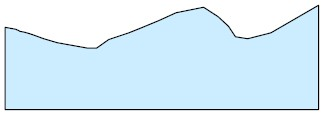
\includegraphics{TeXGraphics/Chapter5Fig.jpg}	
\caption{Area under a curve}	
\label{Chapter5Fig}\end{figure}



\item   Which of the trapezoid rule or Simpson's Rule should give a better approximation to the area under a "nice" function?  Justify your response with an illustration.

\item   Compare and contrast the processes of approximating error with rectangles, trapezoids and Simpson's Rule.

\item   Why is numerical integration important?  Are there any definite integrals you would be faced with now that you would have to use numerical integration to find a value?  What is it about these definite integrals that makes them different than the ones we studied at the beginning of the semester?

\end{enumerate}
